\documentclass[10pt]{beamer}

\usetheme{metropolis}
\usepackage{appendixnumberbeamer}
\usepackage{booktabs}
\usepackage[scale=2]{ccicons}
\usepackage{pgfplots}
\usepgfplotslibrary{dateplot}
\usepackage{xspace}
\usepackage[utf8]{vietnam}
\usepackage[english]{babel}
\usepackage{tabularx}
\usepackage{caption}

% --- CUSTOM COLUMN TYPES ---
\newcolumntype{L}{>{\raggedright\arraybackslash}X}
\newcolumntype{C}{>{\centering\arraybackslash}X}

% --- METROPOLIS THEME CUSTOMIZATION ---
\definecolor{DeepBlue}{RGB}{0, 51, 102}
\setbeamercolor{palette primary}{bg=DeepBlue, fg=white}
\setbeamercolor{progress bar}{fg=DeepBlue}
\setbeamercolor{title separator}{fg=DeepBlue}
\setbeamercolor{structure}{fg=DeepBlue}
\setbeamercolor{normal text}{fg=black}

% --- TITLE INFO ---
\title{Traffic Sign Classification}
\subtitle{Deep Feature Manifolds \& Hybrid SVM Optimization}
\date{Final Project Report --- 2026}
\author{Đỗ Duy Toàn, Vũ Tùng Lâm, Nguyễn Thái An,\\Nguyễn Văn Linh, Phạm Viết Hải Đăng, Tạ Hiếu Nam}
\institute{University of Science and Technology of Hanoi}
\titlegraphic{\hfill
\includegraphics[height=1.5cm]{usth.png}}

\begin{document}

\maketitle

\begin{frame}{Table of contents}
  \setbeamertemplate{section in toc}[sections numbered]
  \tableofcontents[hideallsubsections]
\end{frame}

% --- SECTION 1: INTRODUCTION ---
\section{Introduction}

\begin{frame}[fragile]{Project Objectives}
  \begin{itemize}
    \item \textbf{Goal:} Build a robust traffic sign recognition system for autonomous vehicles.
    \item \textbf{Key Approach:} Bridge the gap between Deep Learning and Support Vector Machines.
    \item \textbf{Innovation:} Investigation of Low-Dimensional (3D) Manifold Classification.
  \end{itemize}
\end{frame}

\begin{frame}{Dataset: GTSRB (10-class Subset)}
    \begin{center}
        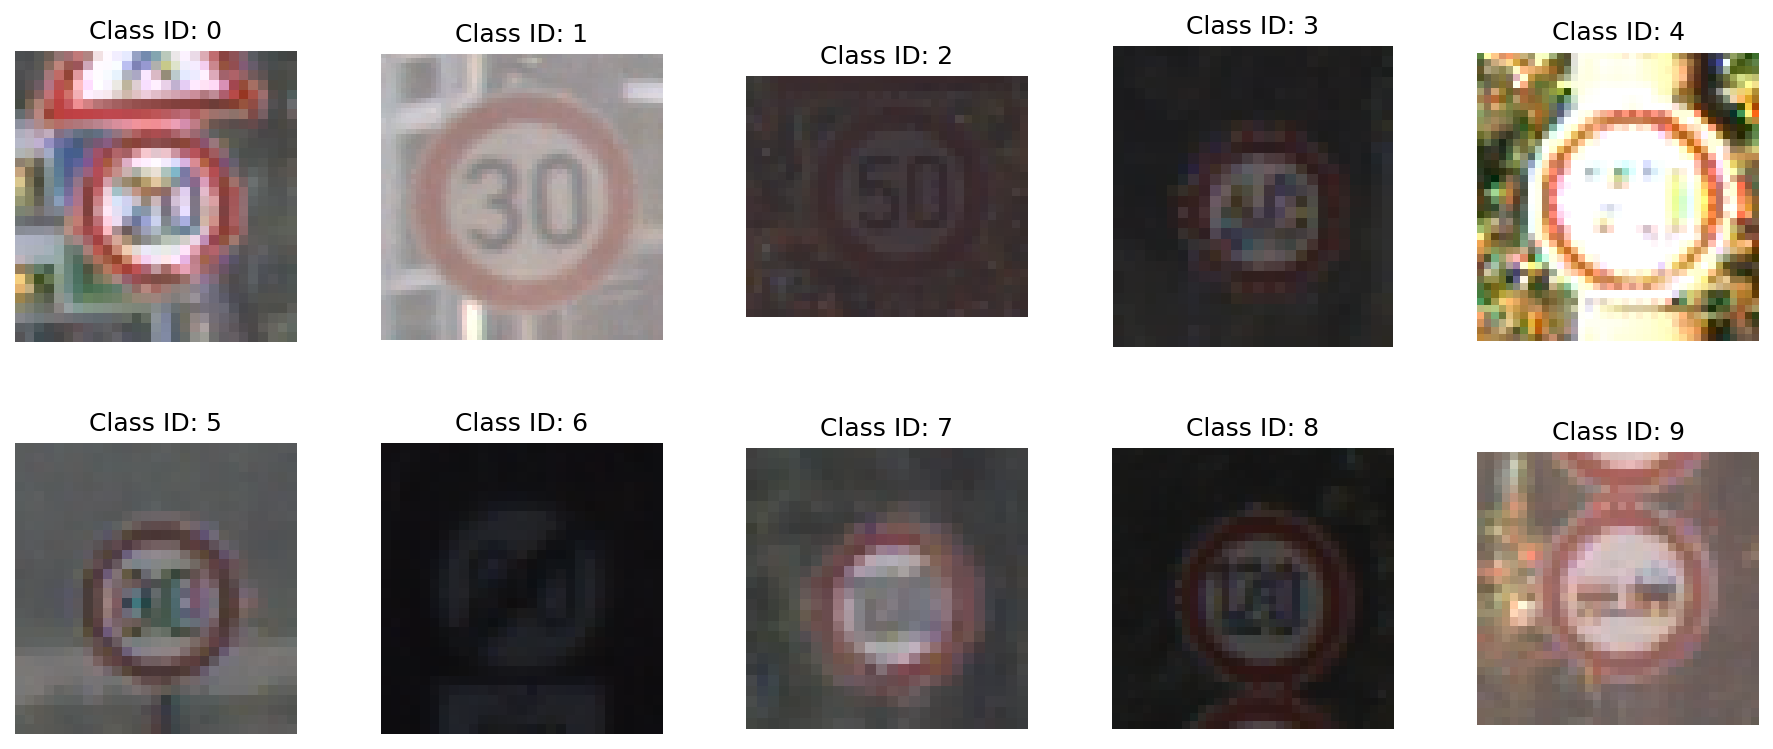
\includegraphics[width=0.7\textwidth]{../reports/figures/dataset_samples.png}
    \end{center}
    \begin{itemize}
        \item Over 10,000 images across 10 distinct traffic sign categories.
        \item Significant scale and illumination variations.
    \end{itemize}
\end{frame}

% --- SECTION 2: METHODOLOGY ---
\section{Methodology}

\begin{frame}{System Pipeline Overview}
    \begin{columns}
        \column{0.45\textwidth}
        \begin{center}
            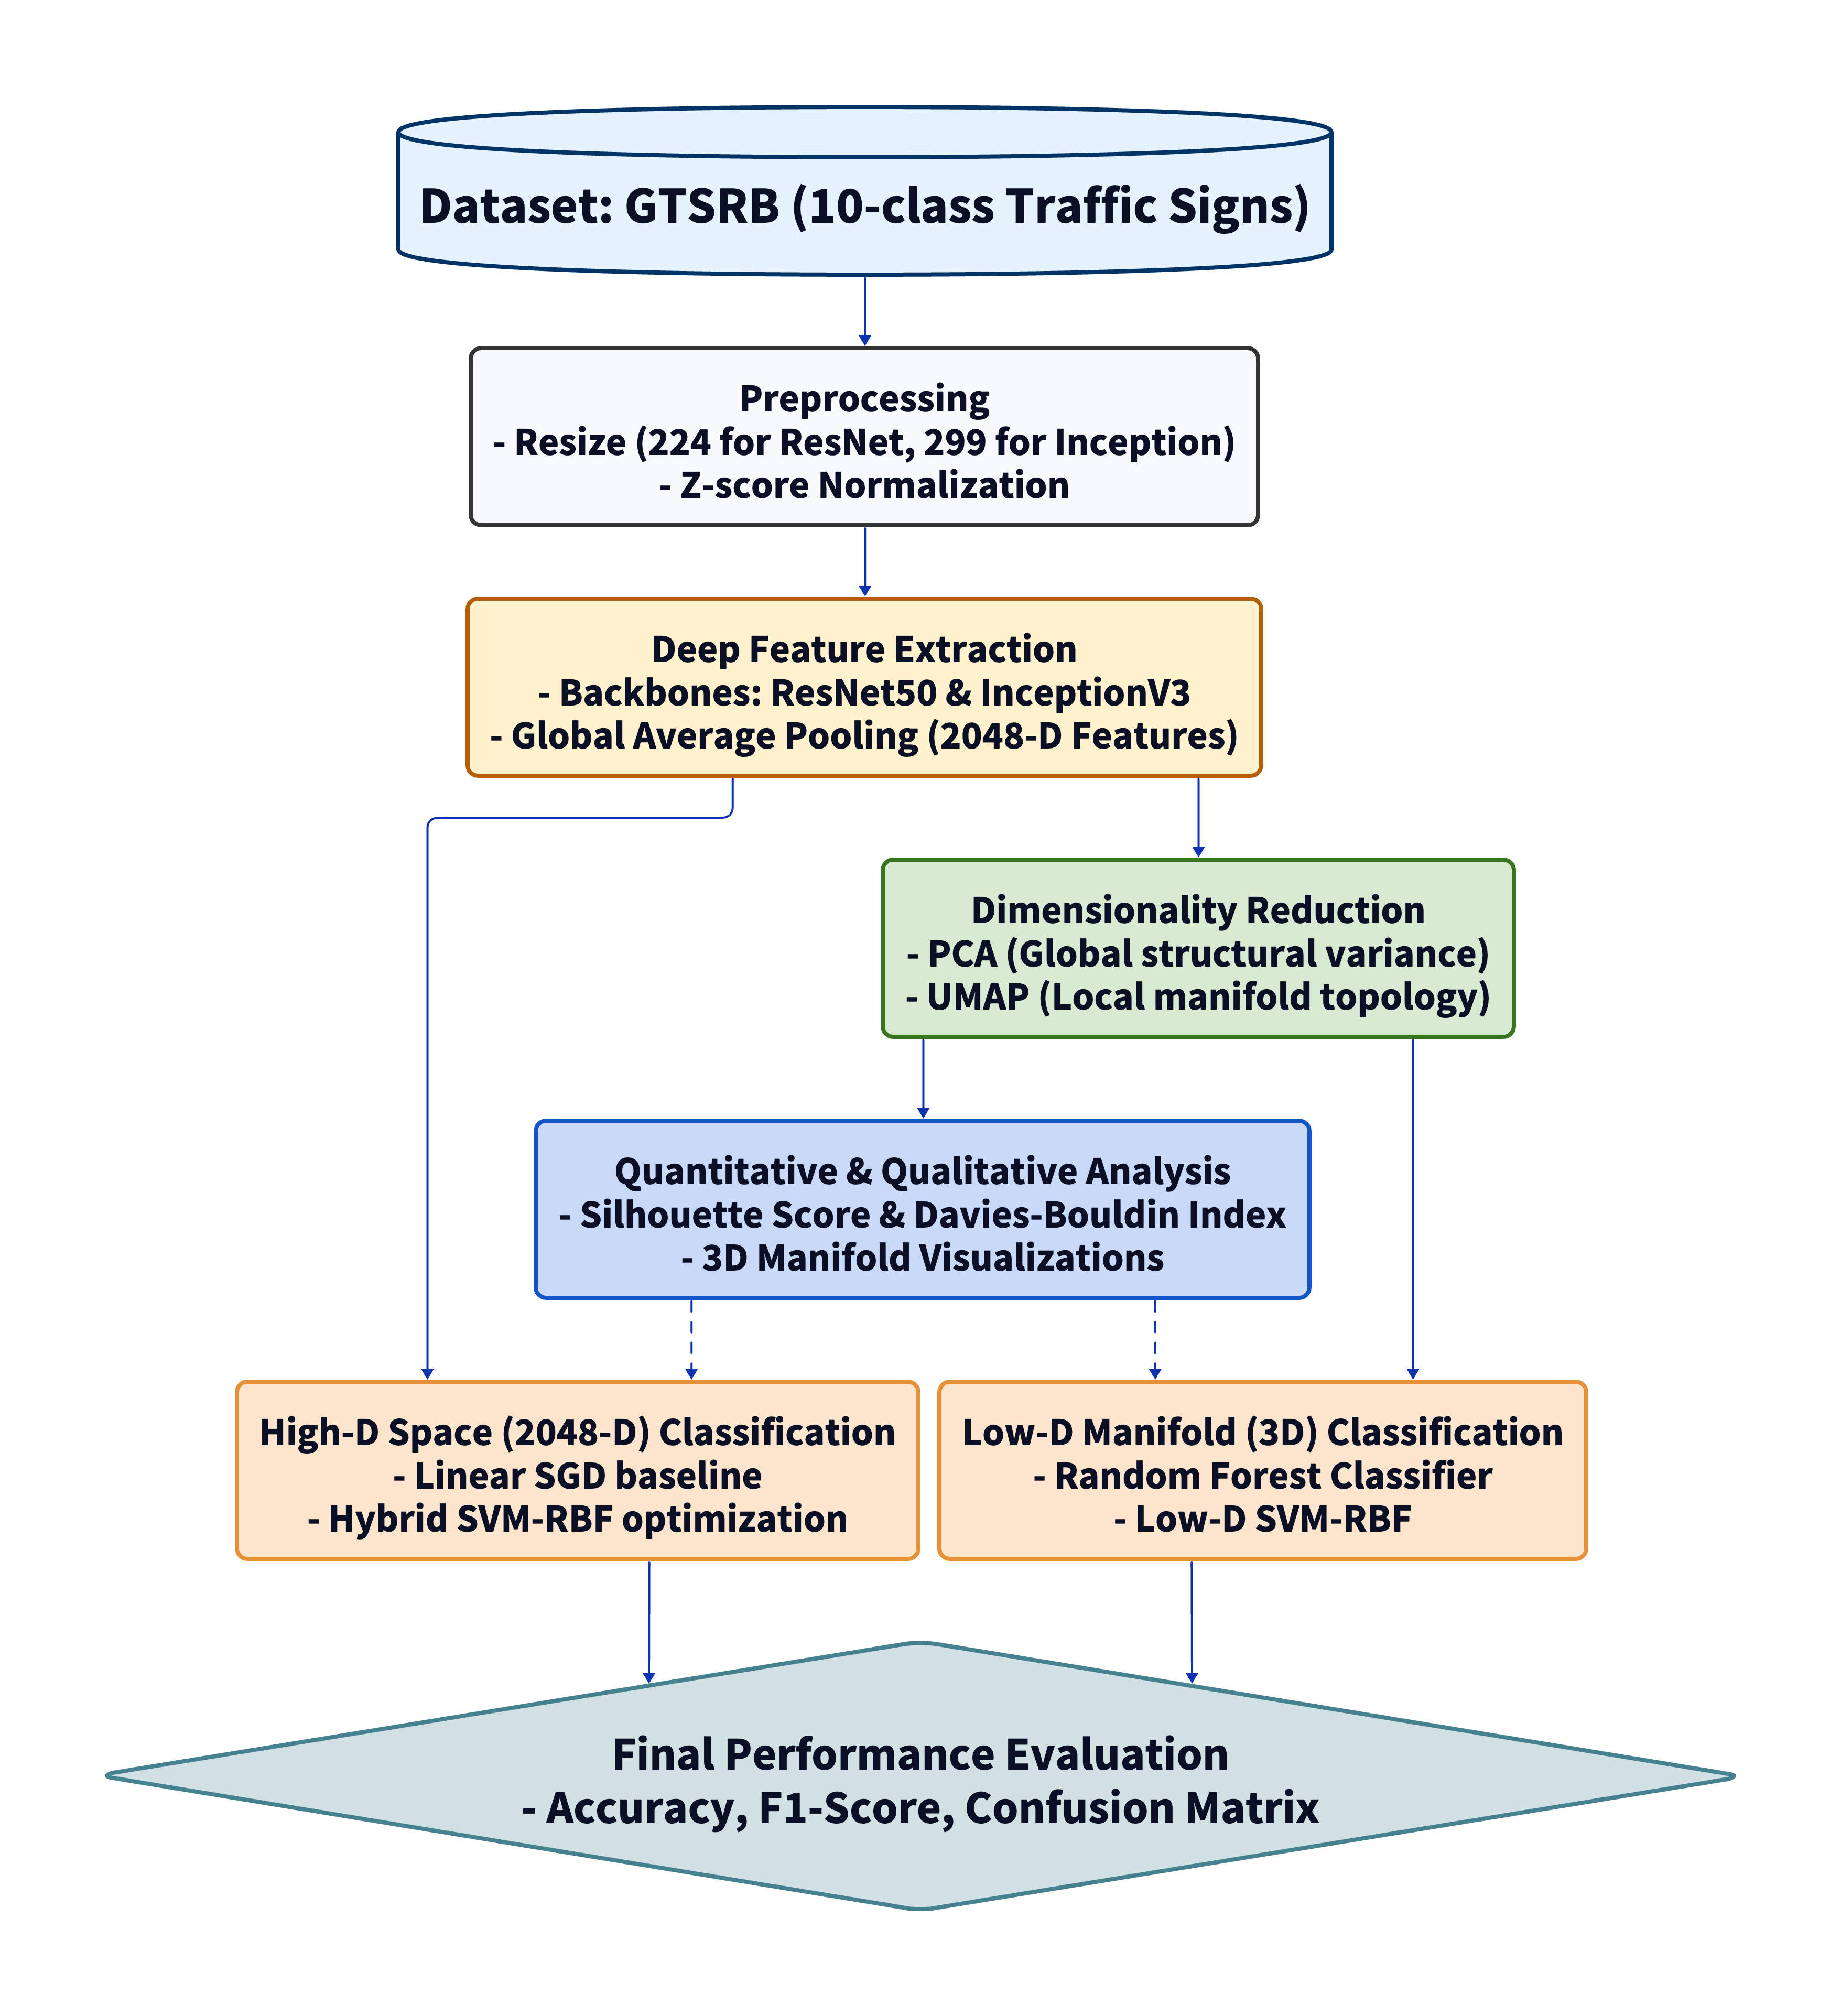
\includegraphics[height=0.75\textheight]{../reports/figures/pipeline_flow.png}
        \end{center}
        
        \column{0.55\textwidth}
        \footnotesize
        \begin{enumerate}
            \item \textbf{Data \& Preprocessing}: Stratified 10-class selection; Z-score normalization.
            \item \textbf{Feature Extraction}: Deep CNN backbones as 2048-D semantic encoders.
            \item \textbf{Geometric Analysis}: Contrast of Global (PCA) vs. Local (UMAP) topology.
            \item \textbf{Dual-Track ML}: Evaluation on High-D space vs. Compressed 3D manifolds.
        \end{enumerate}
    \end{columns}
\end{frame}

\begin{frame}{3D Manifold Visualizations (UMAP)}
    \begin{columns}
        \column{0.5\textwidth}
        \begin{center}
            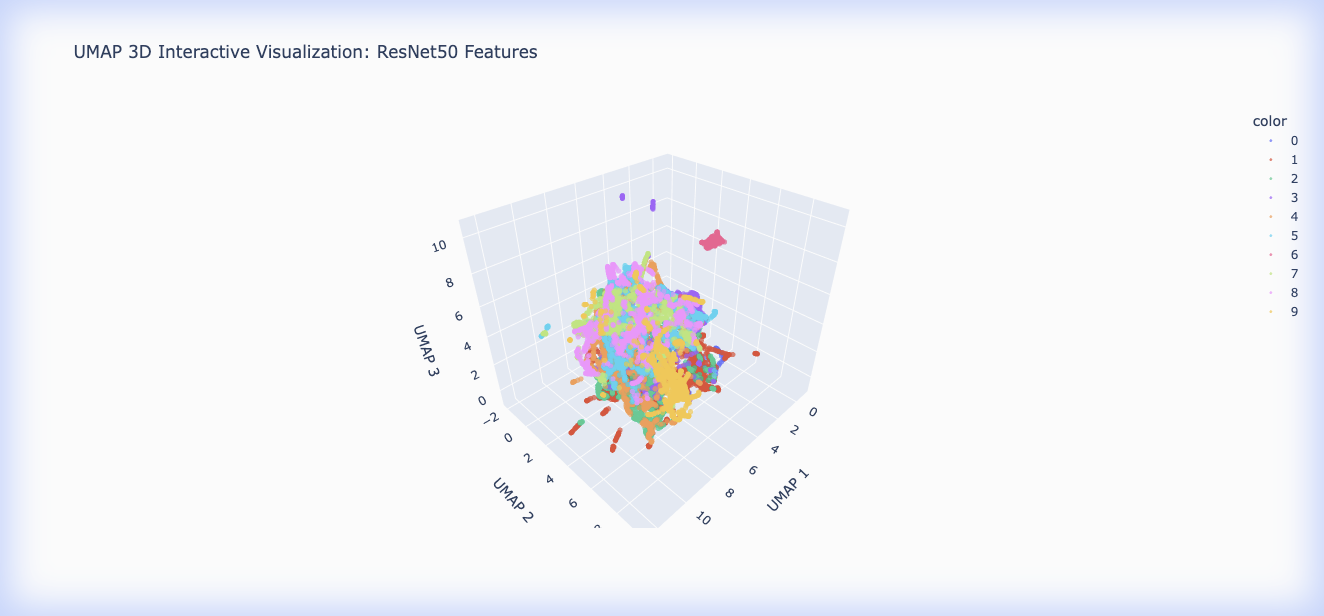
\includegraphics[width=\textwidth]{../reports/figures/umap_3d_resnet50_static.png}
            \small ResNet50 Manifold
        \end{center}
        \column{0.5\textwidth}
        \begin{center}
            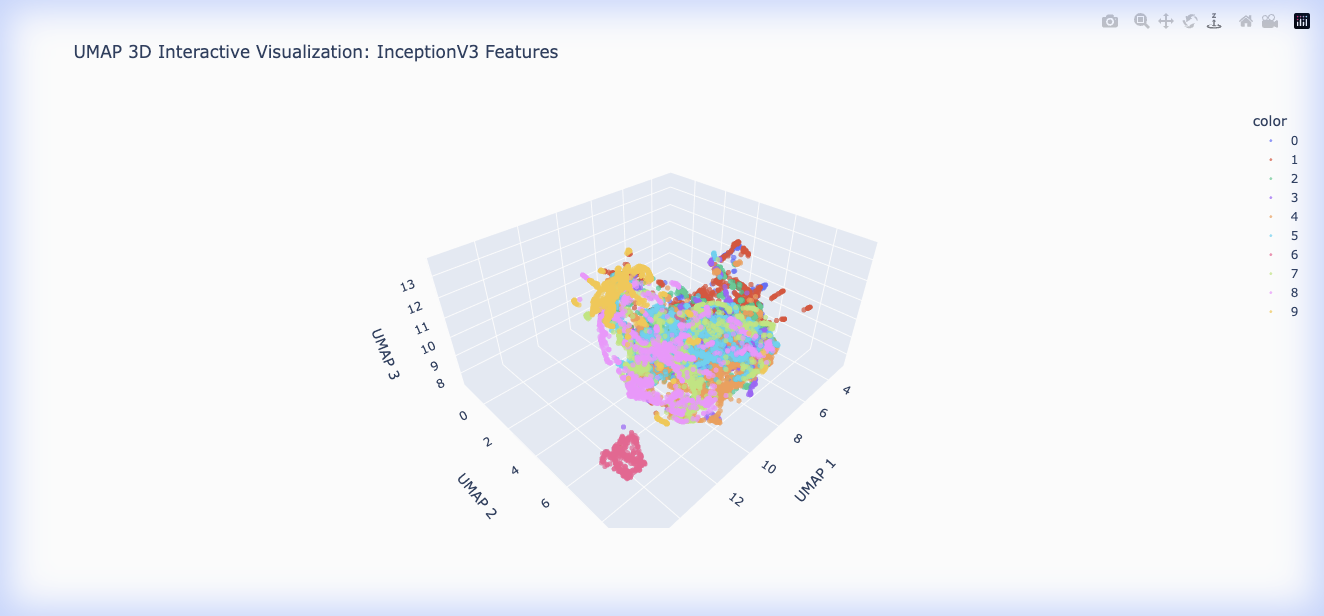
\includegraphics[width=\textwidth]{../reports/figures/umap_3d_inceptionv3_static.png}
            \small InceptionV3 Manifold
        \end{center}
    \end{columns}
    \vspace{0.3cm}
    \textit{UMAP preserves local structures, forming dense semantic clusters.}
\end{frame}

% --- SECTION 3: RESULTS & ANALYSIS ---
\section{Results \& Analysis}



\begin{frame}{Classification in 3D Space}
    \begin{columns}
        \column{0.5\textwidth}
        \begin{itemize}
            \item \textbf{Insight:} Linear models fail in 3D (<35\%).
            \item \textbf{Success:} \textbf{Random Forest} dominates by recursive partitioning.
        \end{itemize}
        
        \begin{table}
            \centering
            \footnotesize
            \begin{tabular}{lc}
                \toprule
                \textbf{3D Classifier} & \textbf{Acc. (R50)} \\
                \midrule
                SGDC (Linear) & 28.94\% \\
                SVM-RBF & 51.74\% \\
                \textbf{Random Forest} & \textbf{82.28\%} \\
                \bottomrule
            \end{tabular}
        \end{table}

        \column{0.5\textwidth}
        \begin{center}
            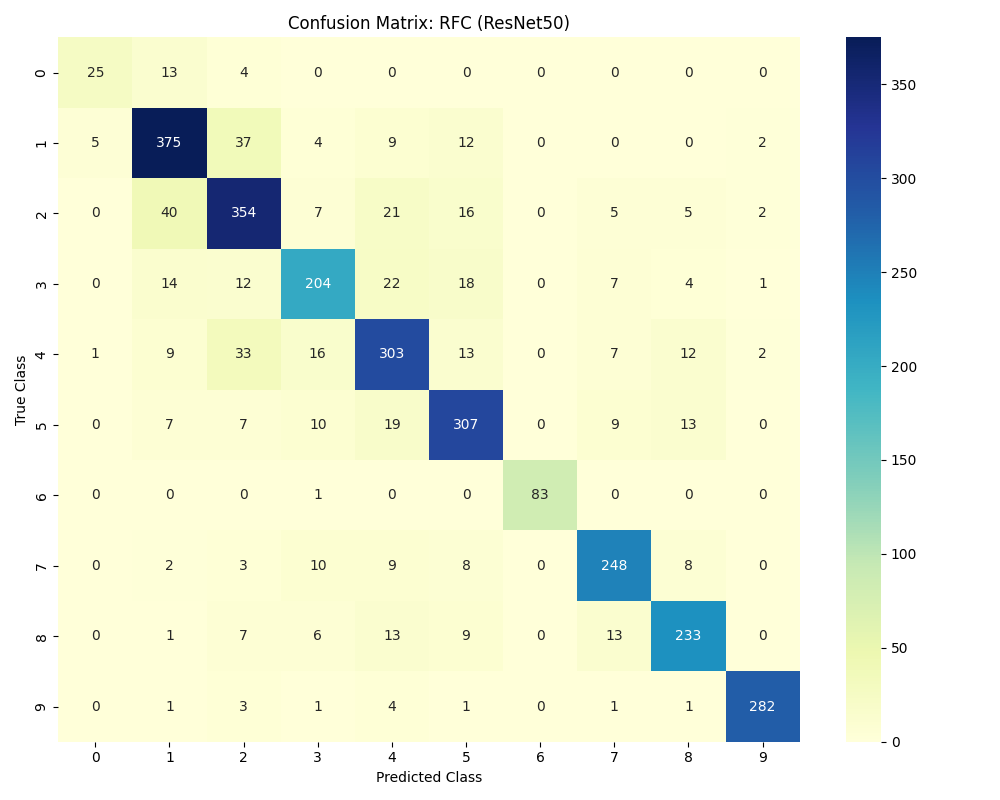
\includegraphics[width=\textwidth]{../reports/experiments/manifold_3d/rfc_resnet50_cm.png}
            \tiny RFC Confusion Matrix (ResNet50 3D)
        \end{center}
    \end{columns}
\end{frame}

\begin{frame}{High-D Classification Results}
    \begin{columns}
        \column{0.45\textwidth}
        \begin{table}
            \centering
            \footnotesize
            \begin{tabularx}{\textwidth}{L C C}
                \toprule
                \textbf{Model} & \textbf{R50} & \textbf{IncV3} \\
                \midrule
                SGD (Lin) & 91.2\% & 88.5\% \\
                \textbf{RBF (Hyb)} & \textbf{95.9\%} & \textbf{97.2\%} \\
                \bottomrule
            \end{tabularx}
            \caption*{Validation Acc.}
        \end{table}
        \footnotesize
        RBF kernels effectively handle the density of deep manifolds, significantly outperforming linear baselines.

        \column{0.55\textwidth}
        \begin{center}
            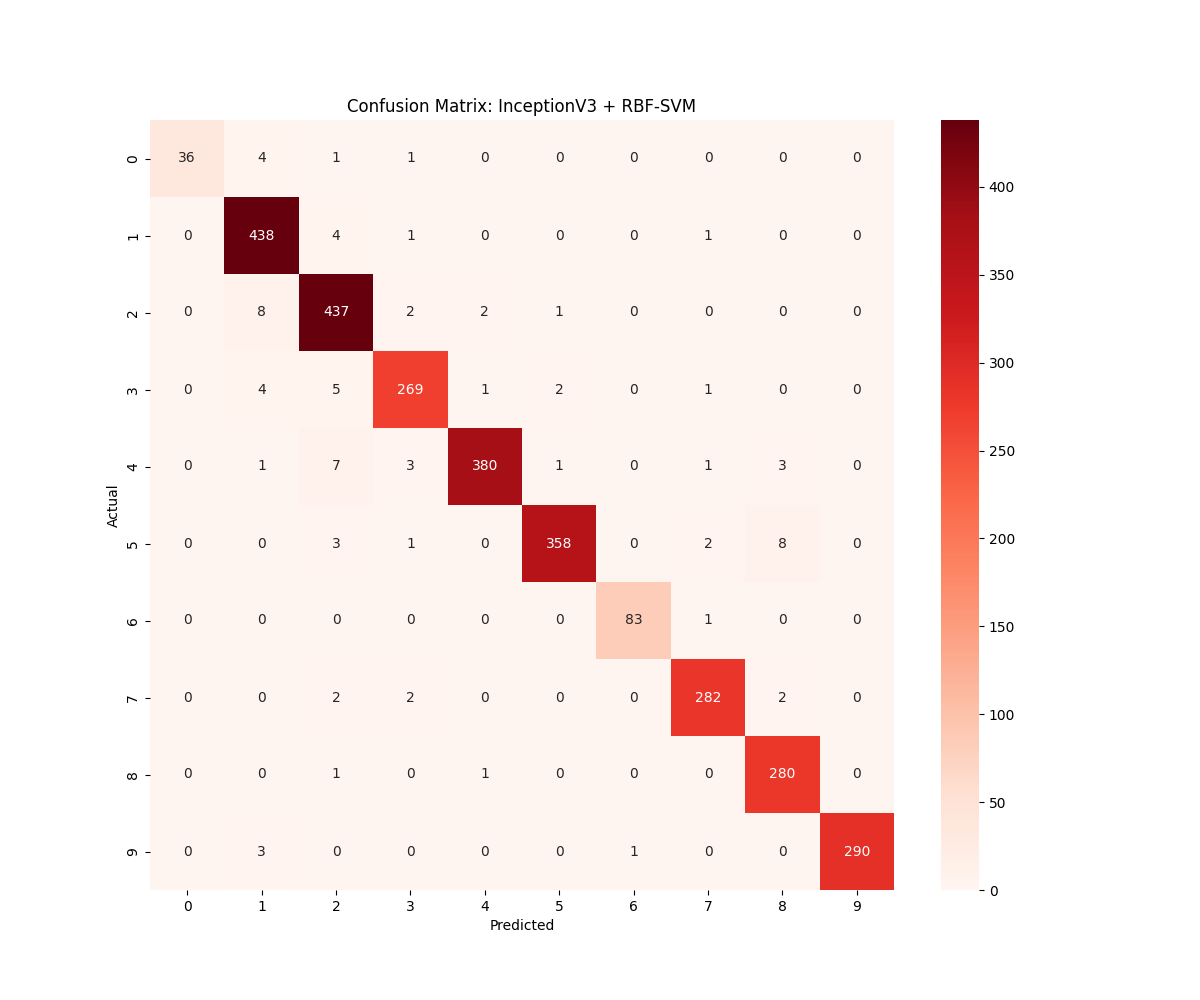
\includegraphics[width=\textwidth]{../reports/performance/inceptionv3_rbf_confusion_matrix.png}
            \tiny Peak Model CM (InceptionV3 + RBF)
        \end{center}
    \end{columns}
\end{frame}

% --- SECTION 4: CONCLUSION ---
\section{Conclusion}

\begin{frame}{Summary}
  \begin{itemize}
    \item Hybrid architectures improve flexibility and performance.
    \item \textbf{RBF kernels} are essential for 2048-D features (achieving up to \textbf{97.24\%} accuracy).
    \item 3D projections retain \textbf{~82\% accuracy}, proving UMAP's density preservation.
  \end{itemize}
  \vspace{0.4cm}
  \begin{center}
      \textbf{GitHub Repository:} \\
      \url{https://github.com/toando0212/final-ml2}
  \end{center}
\end{frame}

\begin{frame}[standout]
  Questions?
\end{frame}

\end{document}
